%!TeX root=./tese.tex
% Artifact & reproduction manifest. Source of truth for provenance is
% progress/results-ledger.md (artifact / command / date / feeds / supersedes
% per result); this appendix is its manuscript-facing distillation.
\chapter{Artifact and Reproduction Manifest}
\label{ap:artifacts}

Nearly every quantitative claim in this document is generated by a
versioned script over archived inputs and recorded in the workspace
results ledger (\texttt{progress/results-ledger.md}). This appendix
distills that ledger: Table~\ref{tab:ap-env} fixes the software
environment, and Table~\ref{tab:ap-manifest} maps each figure and table
to its generating script and primary artifact. Paths are relative to the
workspace root.

\section{Environment}

\begin{table}[htbp]
\centering
\caption{Software environment for the thesis experiments. Full package
freezes live in each virtual environment; the AIC data-collection and
GEMM-validation runs pin the GPU clocks via \texttt{nvidia-smi -lgc
2400,2400 -lmc 14001} (delivered SM 2377--2400\,\si{\mega\hertz}, MEM
\SI{13801}{\mega\hertz}; the AIC cost model itself is parameterised at the
\SI{2407}{\mega\hertz} boost reference), while the phase-E physical encoder anchor ran
single-tenant persistence-mode (delivered SM 2377--2400\,\si{\mega\hertz},
not a hard lock).}
\label{tab:ap-env}
\scriptsize
\setlength{\tabcolsep}{4pt}
\begin{tabular}{@{}lll@{}}
\toprule
Component & Version & Role \\
\midrule
NVIDIA driver / CUDA & 595.71.05 / 13.2 & benchmark node (RTX 5090) \\
vLLM (container) & \texttt{vllm/vllm-openai:v0.22.0} & collection + kernel profiling \\
aiconfigurator & 0.10.0 (editable, data branch) & encoder + LLM cost model \\
ai-dynamo & 1.2.1 wheel / 1.3.0 source & \texttt{dynamo.replay} runtime \\
aiperf & 0.11.0 & live closed-loop client (TTFT/ITL/goodput) \\
cuDF / cuML / CuPy & 26.06 / 26.06 / 14.1.1 & trace EDA (GPU) \\
PyTorch / transformers & 2.12.1 / 5.13.0 & TSFM benchmark + encoder bench \\
chronos-forecasting & 2.3.1 & Chronos-2 \\
matplotlib & 3.11.0 & all figures \\
\bottomrule
\end{tabular}
\end{table}

The two \texttt{dynamo.replay} runtimes matter for reproduction: the
pinned 1.2.1 wheel is the Phase-2 baseline; the 1.3.0 source build runs
AIC timing predictions in-core (Rust) and is used for every calibrated
run from the load sweeps onward (the wheel's per-request Python timing
callback inflated extreme tail maxima only --- documented in
Chapter~\ref{cap:twopool}).

The GPU EDA environment (\texttt{eda/}: cuDF/cuML/CuPy on the RAPIDS
\texttt{cu13} stack) is reproducible from this checkout via its tracked
\texttt{uv} lock (\texttt{eda/\allowbreak uv.lock},
\texttt{eda/\allowbreak pyproject.toml}); its
multi-gigabyte \texttt{.venv} stays gitignored. The aiconfigurator and
ai-dynamo environments are separate virtual environments external to this
checkout, pinned to the principal versions in Table~\ref{tab:ap-env}. The
encoder campaign runs on draft PR~\#1312 through commit \texttt{b55dd0b7};
only the Dynamo live-planner branch remains a local commit.

\section{Supplementary figures}
\label{ap:supp-figs}

\begin{figure}[htbp]
\centering
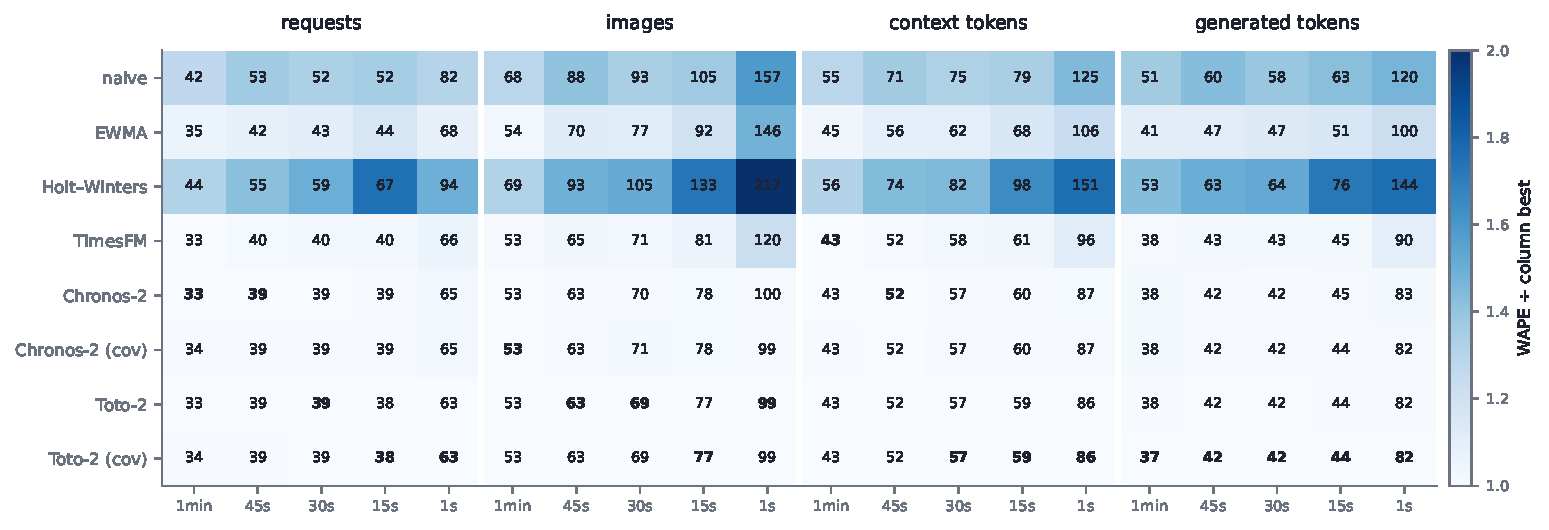
\includegraphics[width=\linewidth]{figuras/pred/pred_wape_heatmap}
\caption{Overall point WAPE (\%, annotated) for every model and every
(signal, resolution) cell on the common span; shading is each cell's WAPE
relative to the best model in its column, bold marks the column best. The
Chronos-2 and Toto-2 rows are near-optimal in every cell and TimesFM close
behind; the baseline rows darken as bins shrink, and column wins split
among the three foundation models by noise-level margins.
Holt--Winters is the worst model in every column --- worse than naive
persistence --- because extrapolating a fitted trend across a 12-step
horizon is precisely wrong for bursty, mean-reverting rates.}
\label{fig:pred-heatmap}
\end{figure}

\begin{figure}[htbp]
\centering
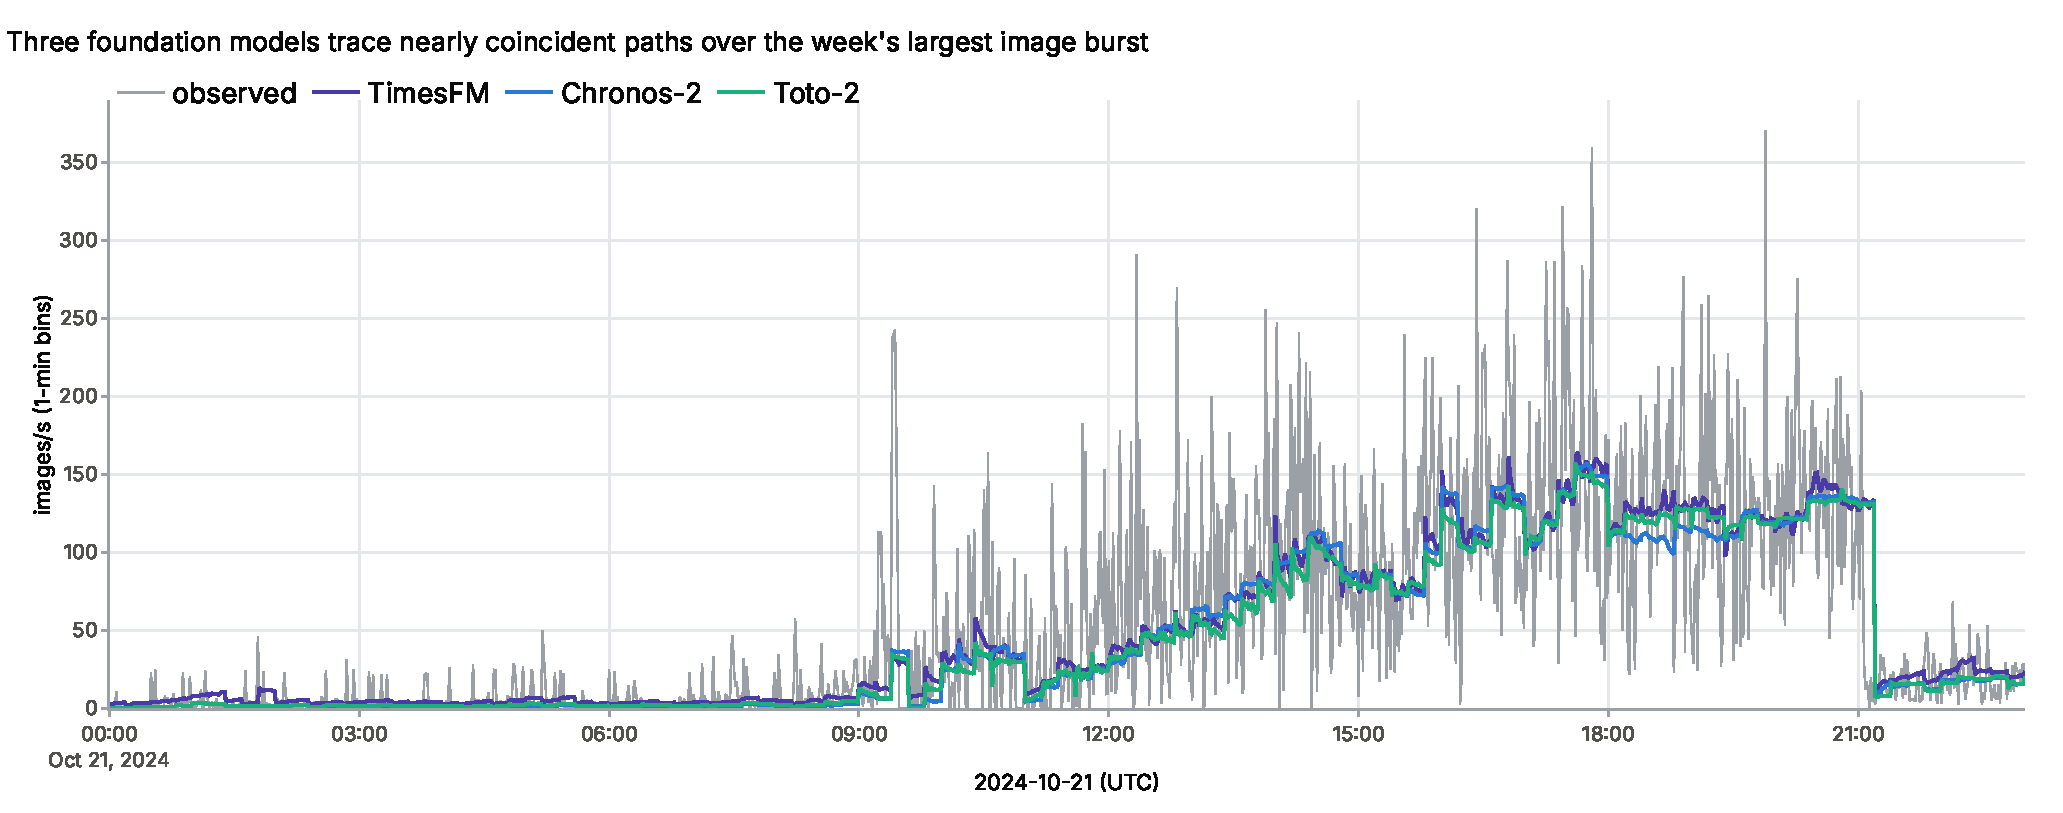
\includegraphics[width=\linewidth]{figuras/pred/pred_models_burst}
\caption{All three foundation models over the same burst (univariate
point paths, \SI{1}{\minute} bins): the paths are nearly coincident ---
riding the plateau, ignoring single-bin spikes, and releasing the regime
within about one tile of its collapse --- the visual form of the
noise-level inter-model spreads in Table~\ref{tab:pred-wape}.}
\label{fig:pred-models}
\end{figure}

\clearpage
\section[Encoder cost model: engine sensitivity]{Execution-engine sensitivity of the encoder cost model}
\label{app:engine-sensitivity}

The batch-axis discrepancy of Section~\ref{sec:aic-model-vs-silicon}
between AIC's composed encoder forward and end-to-end measurement is
predominantly execution-stack-specific --- a property of the
\emph{execution engine} used for measurement more than of the cost model.
This appendix gives the engine-by-engine evidence and the encoder-coverage
contributions returned upstream.

Table~\ref{tab:app-engine} times the same Qwen3-VL vision-tower forward
(bf16, $448^2$, RTX~5090 under an external \texttt{nvidia-smi} clock lock,
target SM \SI{2400}{\mega\hertz}, memory \SI{14001}{\mega\hertz}) under
four execution paths, against AIC's composition. This is a separate
recollection from the Phase-E self-lock attempt of the Environment
section (per-$N$ SM readings 2377--2400 \si{\mega\hertz}, no
memory-clock reading or lock-command log captured).

\begin{table}[htbp]
\centering
\caption{Encoder forward latency (ms) over $N$ images of $448^2$ under
four execution engines vs.\ the AIC composition. HuggingFace and
\texttt{torch.compile} are the \texttt{transformers} module; vLLM is its
own \texttt{Qwen3\_VisionTransformer} with the FlashAttention backend
(the standalone eager vLLM vision-tower implementation). The final column is the ratio of
vLLM---the engine AIC's collected kernels are drawn from---to the
composition.}
\label{tab:app-engine}
\small
\begin{tabular}{rrrrrrr}
\toprule
$N$ & AIC & HF-SDPA & HF-FA2 & vLLM-FA & \texttt{compile} & vLLM/AIC \\
\midrule
1  & 8.2   & 11.3  & 11.2  & 8.0   & 10.1  & 0.98 \\
8  & 43.1  & 58.7  & 54.2  & 42.2  & 48.8  & 0.98 \\
32 & 160.2 & 253.8 & 232.0 & 178.4 & 186.0 & 1.11 \\
64 & 316.4 & 511.6 & 465.6 & 333.6 & 370.6 & 1.05 \\
\bottomrule
\end{tabular}
\end{table}

The four table rows are anchor shapes within the $N{\le}64$-dense sweep;
Figure~\ref{fig:app-engines} plots the engines across the whole batch axis.

\begin{figure}[htbp]
\centering
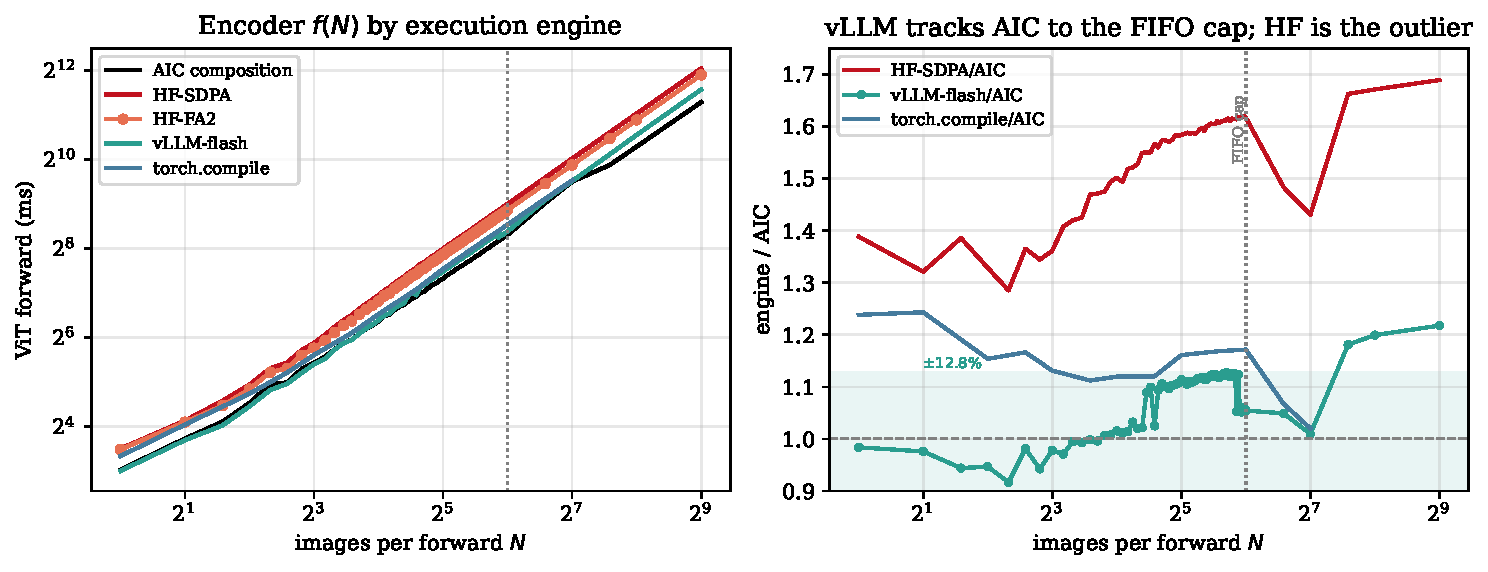
\includegraphics[width=\linewidth]{figuras/aic/aic_fn_engines}
\caption{Dense $f(N)$ for the four execution engines vs.\ the AIC
composition ($448^2$, RTX~5090, external clock lock; $N{\le}64$-dense
sweeps plus off-cap probes, tight CIs, details in the artifact). \emph{Left}: forward latency
(log--log). \emph{Right}: each engine relative to the composition; the
shaded band marks $\pm12.8\%$ and the dotted line the FIFO cap
($N{=}64$). vLLM stays inside the band across the serving regime;
HuggingFace-SDPA climbs to $1.69\times$ by $N{=}512$,
\texttt{torch.compile} between. The AIC curve is the postinfill snapshot
for $N\le128$ and the composed model beyond
(\texttt{aic\_fn\_engines\_aiccurve.csv}).}
\label{fig:app-engines}
\end{figure}

The HuggingFace eager forward (SDPA attention) runs $1.36$--$1.62\times$
above the composition, rising with $N$; FlashAttention-2 recovers part but
leaves the unfused elementwise, DeepStack, and patch-embed overhead
intact, and \texttt{torch.compile} (max-autotune) closes most of the rest
without being either engine's default. vLLM's \emph{own} vision tower
through its FlashAttention backend is the like-for-like anchor --- AIC's
collected operators \emph{are} vLLM's kernels (attention
\texttt{kernel\_source=vllm\_vit\_flash\_attn}, GEMMs vLLM
\texttt{RowParallelLinear}) --- and matches the composition across the
table's anchor shapes. The earlier $1.4$--$1.6\times$ ``gap'' is thus the
HuggingFace$\to$vLLM execution-stack difference; against the engine it
targets, the composition stays within $12.8\%$ across the whole $N\le64$
serving regime (residual up to $+12.7\%$ inside the regime, growing to
$+21.8\%$ only past the FIFO cap at $N{=}64$, reaching that value at the
$N{=}512$ sweep endpoint).

\emph{Scope.} The matched-engine check times eager vLLM's standalone
vision-tower forward on synthetic GPU-resident inputs with randomly
initialised weights (latency is shape-determined, so weight values are not
expected to materially affect these dense-kernel timings): it is the
forward compute, not the complete serving path (image preprocessing,
host-to-device transfer, scheduling, prefill), swept densely over
$N{=}1$--$64$ plus five off-cap probes ($N\in\{96,128,192,256,512\}$). Fed through the encoder FIFO --- the AIC-sized winning week
schedule of Chapter~\ref{cap:closedloop} replayed with $f(N)$ repriced at
the measured vLLM curve --- it leaves the week-scale encoder-delay p99 at
\SI{606}{\milli\second} (from \SI{589}{\milli\second} under AIC),
non-divergent, so the AIC-priced cost ratio carries no separate silicon
penalty. Agreement generalises across resolution ($224^2$--$896^2$),
holding within $15.5\%$ at the two largest, where AIC slightly under-prices
the largest forwards (the beyond-cap drift direction); per-resolution
ratios are archived. A live-worker
confirmation over the full serving path (with weight-loaded provenance)
remains future work. Artifacts:
\texttt{collector\_artifacts/\allowbreak phaseE\_physical\_anchor/\allowbreak}\texttt{vllm\_\allowbreak eager\_\allowbreak dense.\{py,json\}}
(dense sweep), \texttt{vllm\_\allowbreak multires.\{py,json\}} (resolution sweep) and
\texttt{tier2\_\allowbreak vllm\_\allowbreak replay.py} (queue replay).

\paragraph{Encoder-coverage contributions (upstream).} Two gaps in AIC's
encoder path were found and returned to the \texttt{aiconfigurator}
project (draft PR). First, the operator graph omitted the pixel-to-hidden
patch-embedding \textsc{gemm}; a \emph{subsequent} branch added a guarded
\texttt{encoder\_patch\_embed\_gemm} ($\approx0.3\%$ of the forward at
$N{=}64$; the DeepStack mergers were already modelled). This addition
postdates the load-bearing simulation snapshot of the main text, in which
the operator is absent, so the two are consistent. Second, the perf tables blanked the ViT's large-batch shapes --- the
\textsc{gemm} and attention grids stopped well short of the shapes the
ViT queries, so past $N{\approx}42$ the model extrapolated beyond the
grid; ViT-shape rows at large $m$ and attention rows to batch~$512$ were
collected on the 5090 (with a collector out-of-memory fix for a 32\,GB
card). These are additive data/tooling corrections; the committed rows
are preserved exactly.

\section{Figure and table manifest}

{\scriptsize\setlength{\tabcolsep}{3pt}
\begin{longtable}{@{}>{\raggedright\arraybackslash}p{0.30\linewidth}>{\raggedright\arraybackslash}p{0.34\linewidth}>{\raggedright\arraybackslash}p{0.32\linewidth}@{}}
\caption{Manuscript element $\to$ generating script $\to$ primary
artifact. Paths relative to the workspace root; leading directories
shared with the script column are elided from artifacts. EDA scripts run
under \texttt{eda/.venv} (GPU); simulation drivers under the
aiconfigurator venv (converter) and \texttt{ai-dynamo/dynamo/.venv}
(replay, source build).}
\label{tab:ap-manifest}\\
\toprule
Element & Script & Primary artifact \\
\midrule
\endfirsthead
\multicolumn{3}{@{}l}{\scriptsize\emph{(Table~\ref{tab:ap-manifest} continued)}}\\
\toprule
Element & Script & Primary artifact \\
\midrule
\endhead
\bottomrule
\endlastfoot
Fig.~\ref{fig:intro-arch} & (TikZ, in source) & --- \\
Figs.~\ref{fig:eda-ctx-vs-img}--\ref{fig:eda-multires};
Tabs.~\ref{tab:eda-archetypes},~\ref{tab:eda-persistence} &
  \texttt{analysis/trace\_eda/ *.py} &
  \texttt{*\_stats.json} (same dir) \\
Tab.~\ref{tab:pred-wape};
Figs.~\ref{fig:pred-heatmap}--\ref{fig:pred-horizon},
\ref{fig:pred-band}, \ref{fig:pred-models},
\ref{fig:cl-framework-diff} &
  \texttt{predictors/ \{benchmark, precision, figures\_tex\}.py} &
  \texttt{results/*.parquet} (the 4-signal $\times$ 6-model base grid);
  runtime logs
  \texttt{results/logs/} \\
Dynamo shipped-predictor comparison (\S\ref{sec:pred-point}) &
  registry sweep through the same protocol &
  \texttt{predictors/ results\_dynamo/ \{arima,kalman,prophet,
  constant\}\_*.json; comparison\_table.csv} \\
Additive context decomposition (\S\ref{sec:pred-covariates}) &
  structural ablation over the archive &
  \texttt{results/metrics/
  additive\_\allowbreak structural\_\allowbreak ablation.json} \\
Quantile coverage (\S\ref{sec:pred-quantiles}) &
  coverage pass over the archive &
  \texttt{results/metrics/ quantile\_coverage.json} \\
Tab.~\ref{tab:aic-validation} &
  \texttt{collector\_artifacts/ phaseA\_validation/} &
  audit artifacts per phase \\
Tab.~\ref{tab:aic-fn}, Fig.~\ref{fig:aic-fn} &
  \texttt{collector\_artifacts/ phaseB\_batch\_validation/} &
  \texttt{measured\_f\_n\_5x50.csv}; \texttt{aic\_f\_n\_postinfill.csv};
  \texttt{kernel\_ledger\_N\{1,64\}.json} \\
Shape infill (\S\ref{sec:aic-collection}) &
  \texttt{collector\_artifacts/ phaseC\_vit\_shape\_infill/} &
  merged parquets (AIC branch, \texttt{656ac8ca}); row counts
  7{,}679$\to$7{,}760 attn, 34{,}326$\to$34{,}710 GEMM \\
Tab.~\ref{tab:sim-poly-aic} &
  \texttt{simulation/run\_replay.sh} &
  \texttt{results/srcbuild/ llm\_head2k\_*\_src.json} \\
Tab.~\ref{tab:sim-knees}, Fig.~\ref{fig:sim-knees} &
  \texttt{simulation/sweep\_load.py}; \texttt{sweep\_fig.py} &
  \texttt{results/sweeps/ summary.json} \\
235B family transfer (\S\ref{sec:sim-timing}; ITL/TTFT p99, ms: wheel
  $s{=}1$ 87.7/397.7; source 1.3.0 $s{=}1$ 86.2/387.4, $s{=}2$
  210.6/524.0) &
  wheel-era spot check \texttt{simulation/ run\_replay.sh}
  (\texttt{AIC\_TP=8}, \texttt{AIC\_MOE\_TP=8}); source-built ladder
  \texttt{defense/anim/build/ gen\_g3\_32b.py} &
  \texttt{simulation/results/235b/
  llm\_head2k\_\allowbreak aic235btp8\_\allowbreak s\{1,4,16\}.json}
  (wheel era); \texttt{defense/anim/data/g3\_32b/
  reports/235b\_tp8\_s*.report.json} (DB runs
  \texttt{g3\_32b:235b\_\allowbreak tp8\_*}) \\
Fig.~\ref{fig:sim-burst-queue} &
  \texttt{simulation/ burst\_queue\_fig.py} &
  \texttt{results/sweeps/series/ vision\_burst1\_s1.series.json} \\
Cap sensitivity (\S\ref{sec:sim-limitations}) &
  \texttt{workload/trace\_to\_two\_pool.py} &
  \texttt{results/cap\_sensitivity/} \\
Tab.~\ref{tab:base-tp} (iso-cost TP; burst5 archived at $C{=}16$) &
  \texttt{simulation/sweep\_grid.py} (TP cells) &
  \texttt{results/grid/reports/ grid\_llm\_*\_\{N4\_aic,
  N2\_TP2\_aic\}.report.json} \\
Tab.~\ref{tab:cl-ewma} (EWMA calibration loop) &
  EWMA p90 calibration through the identical encoder loop &
  \texttt{verification/results/ ewma\_\{baseline\_*, sweep\}.json} \\
Tabs.~\ref{tab:cl-ledger-enc}--\ref{tab:cl-ledger-joint}
  (request-linked arm set) &
  composed replays joined one-to-one by artifact path &
  provenance store (schema \texttt{provenance}: \texttt{v\_joint\_e2e},
  \texttt{v\_pool\_latency}, \texttt{v\_pool\_cost}) over
  \texttt{simulation/results/} \\
Daily folds (\S\ref{sec:cl-limits}) &
  fold split + per-fold replay &
  \texttt{defense/anim/data/ g4\_folds/folds\_table.md} \\
Hybrid encoder schedule $\max(fc,re)$: aggregate, F1--F7 folds,
  combiner sweep (\S\ref{sec:cl-aggregate}) &
  \texttt{simulation/
  run\_encoder\_\allowbreak hybrid\allowbreak\{,\_folds,\_combos\}.sh};
  combiner \texttt{simulation/ combine\_schedules.py} &
  \texttt{simulation/results/ encoder\_hybrid/}:
  \texttt{\{fc,re,hybrid\}.*} (aggregate),
  \texttt{F6\_\{fc,re,hybrid\}.*}, \texttt{folds/ F\{1..7\}\_*.*},
  \texttt{combos/*.*} (its p90/re cells are byte-identical to the
  \texttt{F6\_*} runs); DB runs \texttt{encoder\_hybrid:*} \\
Tab.~\ref{tab:base-grid} (burst5 $C^{*}$ corrected to 8) &
  \texttt{simulation/sweep\_grid.py} (+35 close-out corner runs);
  burst5 stability correction \texttt{verification/scripts/ burst5\_stability.py} &
  \texttt{results/grid/ grid\_summary.json} (burst5 row superseded by
  \texttt{verification/ rerun-stability-e2e.md}) \\
Reactive planner (\S\ref{sec:base-reactive-llm}) &
  \texttt{simulation/ run\_32\_reactive.sh} &
  \texttt{results/reactive32/ r32\{A,B\}\_*.report.json} \\
Tab.~\ref{tab:cl-triad};
LLM lead sweep + capacity mapping (\S\ref{sec:cl-llm}) &
  \texttt{simulation/ run\_44\_riders.sh};
  \texttt{replay\_with\_forecast.py} &
  \texttt{results/riders44/ \{ladder\_*, fc\_lead*, fc\_scale*,
  tp2knee\_*\}.report.json} \\
Per-window factorial (60-cell p90 headline + p50; $\rho$-rating
  surface, \S\ref{sec:cl-matrix}); Tab.~\ref{tab:base-react-enc} &
  \texttt{simulation/ run\_44\_factorial\_issuetime.py}
  (\texttt{QUANTILE}/\texttt{RHO} env; issue-time, warm{+}strict);
  target-time exploratory grid
  \texttt{\{gen\_cells\_44.py, e2b\_fleet.py\}}; burst4 reactive
  $L{=}165$ supplementary cell
  \texttt{defense/anim/build/ gen\_a2\_fleet.py} &
  \texttt{simulation/results/ factorial\_issuetime/
  factorial\_issuetime\_\allowbreak\{p50\_rho15,
  p90\_rho\{10,15,20,25\}\}\_\allowbreak results.json};
  target-time grid \texttt{results/ results\_44.jsonl};
  supplementary cell \texttt{defense/anim/data/ a2\_runs/
  burst4\_reactive\_\allowbreak L165.jsonl\allowbreak\{,.stats.json\}}
  (DB run \texttt{a2:burst4\_\allowbreak reactive\_L165}) \\
Week-scale surface (\S\ref{sec:cl-aggregate}; quantile-decisive,
  rating-cost) &
  \texttt{simulation/
  run\_44\_week\_\allowbreak surface\_\allowbreak issuetime.py} (96
  issue-time aggregate cells) &
  \texttt{simulation/results/ week\_surface\_issuetime/
  week\_surface\_\allowbreak issuetime\_\allowbreak results.json} \\
Language-pool week replay (\S\ref{sec:cl-llm}: 651\,ms / 518.6 GPU-h;
  p50, Toto, TimesFM, reactive arms) &
  \texttt{simulation/results/ llm\_week/launch.sh} (composed trace +
  winning encoder schedule through the planner) &
  \texttt{llm\_week/ week\_\{fc\_p90, fc\_p90\_toto, fc\_p90\_timesfm,
  fc\_p50, re\}.report.json} \\
Language operating-point calibration: $q\times s$ grid, held-out
  frontier, daily folds (\S\ref{sec:cl-llm}) &
  \texttt{simulation/ run\_lang\_calib.sh} (burst2/burst6 grid);
  \texttt{run\_lang\_calib\_eval.sh} (held-out windows);
  \texttt{run\_lang\_folds.sh} (folds) &
  \texttt{simulation/results/ lang\_qsweep/}:
  \texttt{\{burst2,burst6\}\_\allowbreak
  p\{50,60,70,80,90\}\_\allowbreak s\{2..8\}.report.json},
  \texttt{eval\_\{p50\_s8, p70\_s6, p90\_\{s1,s4,s6\}\}/},
  \texttt{folds\_*/};
  DB runs \texttt{langcalib:*}, \texttt{lang\_qsweep:*} \\
Controller inference cost (\S\ref{sec:cl-ledger-cost}: per-model
  per-tick pricing and feasibility) &
  \texttt{defense/anim/build/ gen\_a16\_controller\_cost.py} &
  \texttt{defense/anim/data/ a16\_controller\_cost/
  \{accounting.\{csv,json\},
  timing\_\allowbreak\{chronos,toto,timesfm\}\_\allowbreak
  \{cpu,cuda\}.json, timing\_arima\_cpu.json, REPORT.md\}} \\
Onset detection (\S\ref{sec:cl-matrix}) &
  \texttt{simulation/ detect\_onsets\_44.py} &
  \texttt{results/riders44/ detection\_delay.json} \\
Tab.~\ref{tab:cl-aggregate} (0.62$\times$ headline is the issue-time
  schedule; \texttt{run\_44\_aggregate.sh} gives the target-time bound) &
  \texttt{simulation/ run\_44\_aggregate\_\allowbreak issuetime.sh}, wrapping
  \texttt{verification/scripts/
  forecast\_\allowbreak schedule\_\allowbreak issuetime.py}
  (\texttt{--strict-rewarm} for the sensitivity); target-time bound from
  \texttt{simulation/ run\_44\_aggregate.sh} &
  under \texttt{simulation/results/}:
  \texttt{aggregate44/
  fc\_p90\_L\{15,30,45,165\}\_\allowbreak issuetime.*},
  \texttt{fc\_p50\_L30\_issuetime.*},
  \texttt{aggregate44\_rho/ *\_issuetime.*} ($\rho$ frontier),
  \texttt{aggregate44\_strict/ \{fc\_p90\_L*, fc\_p50\_L30,
  fc\_p90\_rho20\_L*\}\_strict.*} (re-warm sensitivity) \\
Encoder cold start (Ch.~\ref{cap:intro} n., \S\ref{sec:base-protocol}) &
  \texttt{collector\_artifacts/ phaseD\_cold\_start/} &
  \texttt{trials.jsonl} \\
Tab.~\ref{tab:val-anchor}; live divergences (\S\ref{sec:val-findings}) &
  \texttt{simulation/live51/ worker\_manager.py} (live control plane:
  etcd/NATS, KV router, per-process TP2 mockers, Prometheus, planner) &
  under \texttt{simulation/results/live51/}: offline twins
  \texttt{twin\_fc*, twin\_re*}; live runs
  \texttt{live\_runs/ \{live\_fc, live\_re,
  verify\_flag\}/ \{planner.log.gz, manager.jsonl,
  profile\_export\_aiperf.json\}} \\
Physical encoder anchor (\S\ref{sec:aic-validation}; collected, reported
in Appendix~\ref{app:engine-sensitivity}) &
  \texttt{collector\_artifacts/ phaseE\_physical\_anchor/
  \{bench\_encoder\_anchor, silicon\_in\_loop, silicon\_multiworker\}.py} &
  \texttt{anchor\_sdpa\_*.json; oneworker\_artifact/;
  silicon\_multiworker.json} \\
Matched-engine vLLM dense sweep + queue replay
  (Fig.~\ref{fig:app-engines}, Appendix~\ref{app:engine-sensitivity}) &
  \texttt{collector\_artifacts/ phaseE\_physical\_anchor/
  \{vllm\_eager\_dense, vllm\_multires, vit\_compile\_dense,
  tier2\_vllm\_replay, make\_engine\_fig\}.py} &
  \texttt{vllm\_eager\_dense.json; vllm\_multires.json;
  vit\_compile\_dense.\{json,log\}; merged\_sdpa.csv; merged\_fa2.csv;
  \{winsched,static\_c8\}\_\allowbreak\{ctrl\_aic,\allowbreak
  treatment\_vllm\}.stats.json;
  replay\_provenance.md; figuras/aic/ aic\_fn\_engines.pdf,
  aic\_fn\_engines\_\allowbreak aiccurve.csv} \\
\end{longtable}}

Workspace layout: \texttt{analysis/trace\_eda/} (GPU EDA),
\texttt{predictors/} (TSFM benchmark), \texttt{collector\_artifacts/}
(AIC collection/validation audit trail, one artifact per phase),
\texttt{workload/} (trace-to-two-pool converter, encoder FIFO
simulation), \texttt{simulation/} (sweep/grid/planner drivers and
results), \texttt{tex/} + \texttt{figuras/} (this document). The
collected AIC datasets were contributed upstream as draft PR
ai-dynamo/aiconfigurator~\#1312 (campaign through commit \texttt{b55dd0b7}, pushed and open on
the draft PR).
